\pagebreak

\section{Mandeaften}

\textbf{Sted:} Græsplæne ude foran køkken. \\

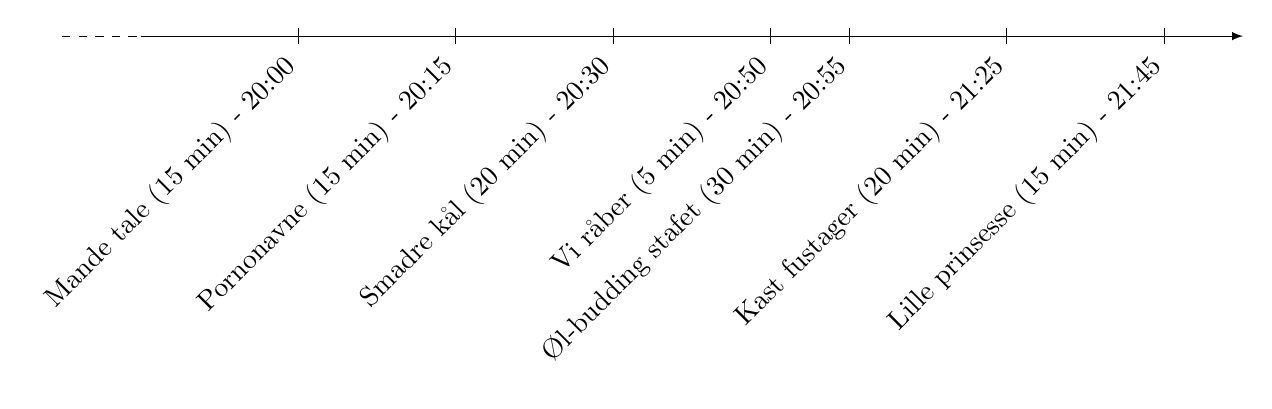
\begin{tikzpicture}
   \draw[-, dashed] (-1,0) -- (0,0);
   \draw[|->, -latex] (0,0) -- (14,0);
   
   \draw[] (2,-0.1) -- (2,0.1);
   \draw (2,0) node[below=7pt,anchor=east,xshift=0,rotate=45] {Mande tale (15 min) - 20:00};
   
   \draw[] (4,-0.1) -- (4,0.1);
   \draw (4,0) node[below=7pt,anchor=east,xshift=0,rotate=45] {Pornonavne (15 min) - 20:15};
   
   \draw[] (6,-0.1) -- (6,0.1);
   \draw (6,0) node[below=7pt,anchor=east,xshift=0,rotate=45] {Smadre kål (20 min) - 20:30};
   
   \draw[] (8,-0.1) -- (8,0.1);
   \draw (8,0) node[below=7pt,anchor=east,xshift=0,rotate=45] {Vi råber (5 min) - 20:50}; 
   
   \draw[] (9,-0.1) -- (9,0.1);
   \draw (9,0) node[below=7pt,anchor=east,xshift=0,rotate=45] {Øl-budding stafet (30 min) - 20:55}; 
   
   \draw[] (11,-0.1) -- (11,0.1);
   \draw (11,0) node[below=7pt,anchor=east,xshift=0,rotate=45] {Kast fustager (20 min) - 21:25}; 
   
   \draw[] (13,-0.1) -- (13,0.1);
   \draw (13,0) node[below=7pt,anchor=east,xshift=0,rotate=45] {Lille prinsesse (15 min) - 21:45}; 
\end{tikzpicture}

\textbf{Mande tale:} \Farav holder mande talen. \\
\textbf{Pornonavne:} Vi finder pornonavne, man skal hedde resten af mandeaften \\
\textbf{Øl-budding staffet:} Vi løber ned, spiser øl-budding (plus løg og snackbacon) \\ 
\textbf{Kaster fustager:} Hvem kan kaste længest? \\
\textbf{Lille prinsesse:} Se næste side

\textbf{Husk:} Som rigtige gentlemen taber vi :-(

\textbf{Materiale liste}
\begin{itemize}
  \item Kål + Bat
  \item Dæk % så man kan sparke lidt til det
  \item Ting til at åbne øl med:
  \begin{itemize}
    \item Sav/hammer/værktøj
    \item Avis
    \item Krokketkugle
  \end{itemize}
  \item Plastik-kop til øl-budding (skal helst kunne tåle ca $50\,^{\circ}\mathrm{C}$ varmt vand)
\end{itemize}

\pagebreak
\textbf{Mine Herrer!}\\
- Vi er samlet her i dag, \underline{\textbf{UDEN KVINDER!}} Men hvorfor er vi det? Det er vi fordi vi har en historisk forpligtelse til at samles i patriarkiets hellige navn, for at praktisere den vigtigst og fornemste af de ting, der figurerer på den nærmest endeløse liste over ting, som mænd er i stand til, og som kvinder ikke er. Nej, vi snakker ikke om at køre bil, spille boldspil eller tage beslutninger. Vi snakker om at diskutere \textbf{VIGTIGE TING! (VIGTIGE TING! VIGTIGE TING!)}\\
- Det hele startede i år 336 f. Kr., hvor Alexander den Store samlede sine mænd og drog på erobringstogt \underline{\textbf{UDEN KVINDER}}. Men hvorfor gjorde han det? For at diskutere \textbf{VIGTIGE TING! (VIGTIGE TING! VIGTIGE TING!)}\\
- I år 58 f. Kr. gjorde en mand ved navn Julius Cæsar ham kunststykket efter. Han samlede ligeledes sine mænd og tog på erobringstogt \underline{\textbf{UDEN KVINDER}}. Men hvorfor gjorde han det? For at diskutere \textbf{VIGTIGE TING! (VIGTIGE TING! VIGTIGE TING!)}\\
- Så når vi frem til Jesus. Han var kendt som lidt af en blød sandalklædt metromand, der var god mod kvinder og dyr. Men da lokummet brændte samlede han sine desciple til nadver \underline{\textbf{UDEN KVINDER}} (fuck af, Dan Brown). Men hvorfor gjorde han det? For at diskutere \textbf{VIGTIGE TING! (VIGTIGE TING! VIGTIGE TING!)}\\
- Hunnerkongen Attila samlede i 430 sine mongolske frænder og tog ud for at plyndre og hærge og voldtage. Dette gjorde de \underline{\textbf{UDEN KVINDER}}. Men hvorfor gjorde de det? For at diskutere \textbf{VIGTIGE TING! (VIGTIGE TING! VIGTIGE TING!)}\\
- I år 600 samlede en mand ved navn Kong Arthur sine riddere omkring et bord, der havde samme smukke form som ølmaver og testikler. Det foregik naturligvis \underline{\textbf{UDEN KVINDER}}. Men hvorfor gjorde han det? For at diskutere \textbf{VIGTIGE TING! (VIGTIGE TING! VIGTIGE TING!)}\\
- I år 800 var det så vores hornklædte forgængere, vikingerne, der drak sig i mjød-hegnet, og tog ud i verden for at plyndre og hærge og voldtage. Det gjorde de \underline{\textbf{UDEN KVINDER}}. Men hvorfor gjorde de det? For at diskutere \textbf{VIGTIGE TING! (VIGTIGE TING! VIGTIGE TING!)}\\
- Så vil der ske om 600 år. Nemlig i år 1992, hvor den største mand af dem alle, Richard Møller Nielsen, samlede sine mænd og drog til Sverige for at vise hele verden hvordan rigtige mænd spiller fodbold. Ikke noget med fesne, langhårede, metroseksuelle, skabagtige driblekonger med hestetænder. Nej, rigtige mænd får bolden frem af banen ved at sparke HÅRDT og LANGT! Derfor drog han til Sverige uden angribere, og uden offensive midtbanespillere, men vigtigere endnu \underline{\textbf{UDEN KVINDER}}. Men hvorfor gjorde han det? For at diskutere \textbf{VIGTIGE TING! (VIGTIGE TING! VIGTIGE TING!)}\\
- Op gennem tiderne har kvinder mødtes uden mænd for at diskutere ting som strikkeopskrifter, balsamicoeddike, Paradise Hotel, nuancer af baige og hvilken håndcreme, der er bedst efter en lang dag med opvask og rengøring. Er det vigtige ting? (NEJ!!)\\
- Når mænd derimod igennem historien har mødtes \underline{\textbf{UDEN KVINDER}}, nøjagtig som vi i dag mødes og mænd ud i al fremtid vil mødes, bliver verdensordenen skabt, universets gåder afdækket, bajere drukket og peniser målt og sammenlignet. Men først og fremmest bliver der diskuteret..\\
\textbf{VIGTIGE TING!! VIGTIGE TING!! VIGTIGE TING!!}
\pagebreak
